\chapter{{Implementacja programowa systemu}}
\label{chapter:implementacja}

W niniejszym rozdziale pokazane zostały etapy budowania aplikacji. Poszczególne części rozdziału zawierają kolejno diagramy, opis budowy aplikacji oraz zrzuty ekrany gotowej aplikacji z podziałem na funkcjonalności.

\section{{Diagram klas}}

\begin{figure}[h!]
  \centering
  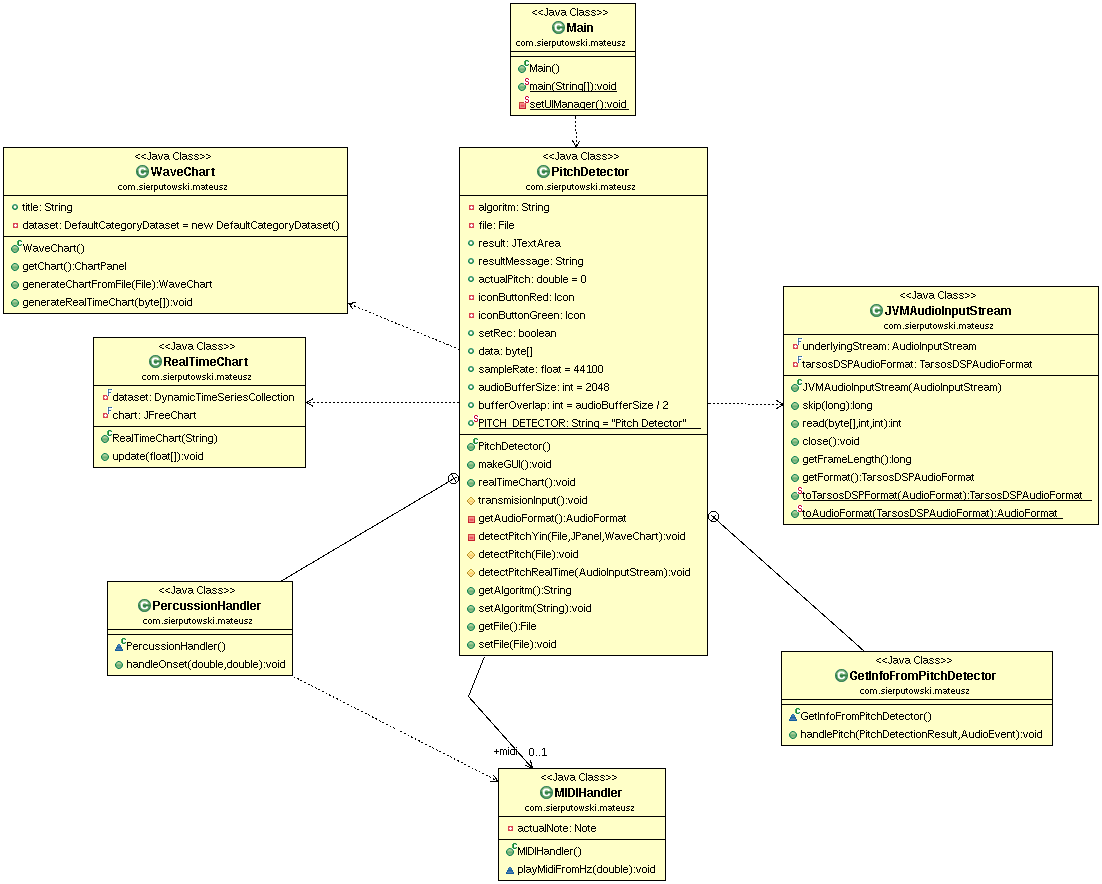
\includegraphics[width=0.9\linewidth]{rys/diagram1}
  \caption{Diagram klas.}
  \label{diagram_klas}
\end{figure}

Diagram na rysunku \ref{diagram_klas} przedstawia klasy użyte w tej pracy inżynierskiej. Główną klasą aplikacji jest klasa PitchDetector. Nazwa tej klasy odzwierciedla również nazwę aplikacji. Jest to główna klasa zawierająca interface graficzny użytkownika. Zawiera również obiekty obsługujące większość funkcjonalności aplikacji. Zawiera również niezbędne do poprawnego działania aplikacji ustawienia domyślne. 


Kolejną klasą zawartą w diagramie jest klasa WaveChart. Klasa ta jest odpowiedzialna za generowanie wykresów. Jest ograniczona jedynie do tworzenia wykresów na podstawie plików wczytanych z dysku. Aby rozszerzyć funkcjonalność, została również stworzona klasa odpowiedzialna za generowanie wykresów w czasie rzeczywistym z przekazywanego strumienia danych o nazwie RealTimeChart. Do obsługi strumieni danych oprócz standardowych bibliotek Javy została wykorzystana klasa JVMAudioInputStream. W celu realizacji jednego z dwóch głównych celów aplikacji zostały stworzone dwie klasy, kolejno GetInfoFromPitchDetector oraz PercussionHandler. Pierwsza z nich jest odpowiedzialna za wykrywanie tonów, druga zaś wykrywa rozpoczęcie trwania tonu w czasie. Aby zrealizować drugi cel aplikacji, użyta została klasa MIDIHandler, która zawiera obsługę protokołu MIDI.







\section{{Diagramy sekwencji}}


\begin{figure}[h!]
  \centering
  \includegraphics[width=1\linewidth]{rys/diagramSec1}
  \caption{Odtwarzanie dźwięku MIDI na podstawie wykrytego tonu z pliku.}
  \label{diagram1}
\end{figure}


\begin{figure}[h!]
  \centering
  \includegraphics[width=1\linewidth]{rys/diagramSec2}
  \caption{Odtwarzanie dźwięku MIDI w czasie rzeczywistym.}
  \label{diagram2}
\end{figure}

\begin{figure}[h!]
  \centering
  \includegraphics[width=1\linewidth]{rys/diagramSec3}
  \caption{Wykrywanie tonu muzycznego z wczytanego pliku.}
  \label{diagram3}
\end{figure}
\newpage

\section{{Opis działania aplikacji}}

W tym rozdziale zostanie omówione działanie aplikacji. Sposób poruszania się po niej oraz obsługi.


Na rysunku \ref{app} zamieszczono zrzuty ekranu ukończonej aplikacji.

\begin{figure}[h!]
  \centering
  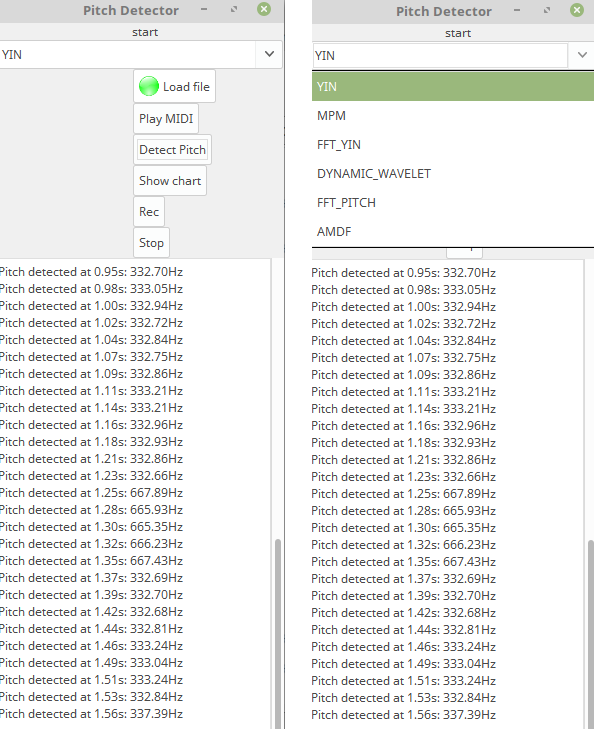
\includegraphics[width=0.5\linewidth]{rys/zrzut1}
  \caption{Zrzut ekranu aplikacji.}
  \label{app}
\end{figure}


Na zrzucie ekranu został przedstawiony interfejs graficzny użytkownika. Do wykonania GUI został wykorzystany pakiet Swing. W górnej części aplikacji znajdują się przyciski funkcjonalne, poniżej został wykorzystany komponent Text Area, który służy do wyświetlania informacji generowanych przez program. Został przedstawiony sposób wyboru algorytmu, który ma posłużyć do wykrywania tonu. Wykorzystany został również mechanizm obsługujący ładowanie plików z dysku.

Głównym mechanizmem do wykrywania częstotliwości jest autokorelacja zrealizowana za pomocą kodu przedstawionego na rysunku \ref{kod1}

\begin{figure}[h!]
  \centering
  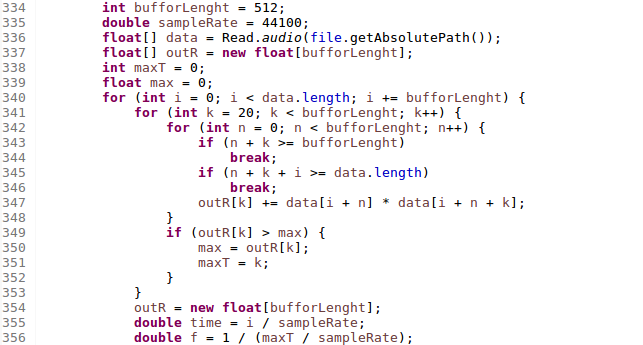
\includegraphics[width=0.9\linewidth]{rys/kod1}
  \caption{Kod wykonujący algorytm autokorelacji}
  \label{kod1}
\end{figure}
W dwóch pierwszych liniach kodu z rys. \ref{kod1} zostają ustawione parametry: wielkości bufora oraz częstotliwość próbkowania. Następnie została użyta metoda Read.audio z dedykowanej biblioteki do obsługi plików w formacie Wave. Metoda ta zwraca dane w formie tablicy float. Kolejno w następnych liniach znajdują się trzy pętle. Pierwsza z nich odpowiada z podział danych na mniejsze partie względem wielkości ustawionego bufora. Kolejne dwie realizują algorytm autokorelacji. Zostaje również wykonany warunek wyszukujący maksimum funkcji w celu odnalezienia dominującego piku. Na końcu głównej zewnętrznej pętli ustawiony zostaje czas oraz poszukiwana częstotliwość.

Do wykrywania tonu w czasie rzeczywistym został wykorzystany kod na rysunku \ref{input}. Wartości próbek zapisywane są do bufora pamięci o rozmiarze 2048, a następnie przekazywane w głównej pętli do funkcji analizującej.
\begin{figure}[h!]
  \centering
  \includegraphics[width=1\linewidth]{rys/input}
  \caption{Kod umożliwiający przetwarzanie w czasie rzeczywistym}
  \label{input}
\end{figure}

\newpage

Obsługa protokołu MIDI została zrealizowana za pomocą kodu zamieszczonego na rysunku \ref{kodMIDI}.

\begin{figure}[h!]
  \centering
  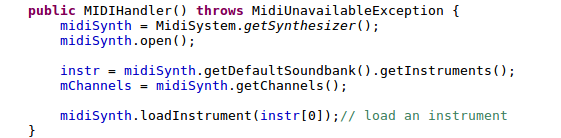
\includegraphics[width=0.9\linewidth]{rys/kodMIDI}
  \caption{Kod obsługujący protokół MIDI}
  \label{kodMIDI}
\end{figure}
Odtworzenie dźwięku oraz ustawienia zostały przedstawione na rysunku \ref{kodMIDI2}.

\begin{figure}[h!]
  \centering
  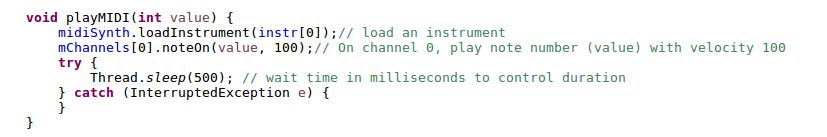
\includegraphics[width=0.9\linewidth]{rys/kodMIDIPlay}
  \caption{Kod obsługujący protokół MIDI}
  \label{kodMIDI2}
\end{figure}
